%! TEX roots = thesis.tex
\documentclass[12pt, titlepage, twoside, openright, usernames, dvipsnames]{thesis}
\title{First-Principles and Machine Learning Investigations into the Atomic and
       Mechanical Properties of Cement Hydrates}
\author{Juan Gabriel Balarezo-Balarezo}
\supervisor{\textbf{Advisor:} Prof. Dr. Henry Pinto Esparza.}

\degree{Physicist}
\discipline{Physics}
\university{Yachay Tech University}
\thesistype{research thesis}

\DeclareMathOperator{\Imag}{Im}
\DeclareMathOperator{\Real}{Re}
\DeclareMathOperator{\Tr}{Tr}
\newcommand{\eF}{\varepsilon_{\textrm{F}}}
\newcommand{\eVBM}{\varepsilon_{\textrm{VBM}}}
\newcommand{\eCBM}{\varepsilon_{\textrm{CBM}}}
\newcommand{\Hmat}{\mathcal{H}}
\newcommand{\Smat}{\mathcal{S}}
\newcommand{\Vmat}{\mathcal{V}}
\newcommand{\Jmat}{\mathcal{J}}
\newcommand{\Tmat}{\mathcal{T}}
\newcommand{\BigO}{\mathcal{O}}
\newcommand{\Lop}{\mathscr{L}}
\newcommand{\Scalpha}{S_{\!C\alpha}}
\newcommand{\Sc}{S_{\!C}}
\newcommand{\Salpha}{S_{\!\alpha}}
\newcommand{\rv}{\textbf{r}}
\newcommand{\Rv}{\textbf{R}}
\newcommand{\kv}{\textbf{k}}
\newcommand{\Kv}{\textbf{K}}
\newcommand{\av}{\textbf{a}}
\newcommand{\bv}{\textbf{b}}
\newcommand{\Bv}{\textbf{B}}
\newcommand{\ev}{\textbf{e}}
\newcommand{\evh}{\hat{\textbf{e}}}
\newcommand{\Ev}{\textbf{E}}
\newcommand{\dv}{\textbf{d}}
\newcommand{\qv}{\textbf{q}}
\newcommand{\Fv}{\textbf{F}}
\newcommand{\Gv}{\textbf{G}}
\newcommand{\hv}{\textbf{h}}
\newcommand{\Tv}{\textbf{T}}
\newcommand{\Cv}{\textbf{C}}
\newcommand{\xv}{\textbf{x}}
\newcommand{\dr}{d^3\rv}
\newcommand{\new}[1]{\textcolor{red}{#1}}
\newcommand{\note}[1]{\textbf{[\textcolor{red}{#1}]}}
\definecolor{RED}{RGB}{1,0,0} %% Error Message avoidance
\newcommand{\Gf}{\mathcal{G}}

\newcommand{\old}[1]{}
\newcommand{\commentout}[1]{}
\theoremstyle{definition}
\newtheorem{theorem}{Theorem}
\theoremstyle{definition}
\newtheorem{definition}{Definition}
\newcommand*\rfrac[2]{{}^{#1}\!/_{#2}}

\usepackage{anysize} % to set up document margins
\marginsize{2cm}{2cm}{2cm}{2cm}
\usepackage{epigraph}
\usepackage[toc,page]{appendix}
\usepackage{tikz}
\usetikzlibrary{shapes.geometric, arrows}
\usepackage{float}
\usepackage{enumitem}
\setlist[enumerate]{itemsep=0mm}
\usepackage{booktabs}
\usepackage[table,xcdraw]{xcolor}
\usepackage{subfigure}
\usepackage[euler]{textgreek}
\usepackage{tablefootnote}
\usepackage{pdfpages}


\graphicspath{{../figures/}}
\usepackage[symbol]{footmisc}

\setcounter{tocdepth}{3}
\setcounter{secnumdepth}{3}
\setlength\epigraphwidth{8cm}
\setlength\epigraphrule{0pt}
% List of abbreviations in the thesis
% Duncan Mowbray <dmowbray@yachaytech.edu.ec>
\newacronym{PCE}{PCE}{power conversion efficiency}
\newacronym{UV}{UV}{ultraviolet spectral region}
\newacronym{VIS}{VIS}{visible spectral region}
\newacronym{IR}{IR}{infrared spectral region}
\newacronym{NIR}{NIR}{near infrared spectral region}
\newacronym{OPV}{OPV}{organic photovoltaic}
\newacronym{P3HT}{P3HT}{poly(3-hexylthiophen-2,5-diyl)}
\newacronym{P3MT}{P3MT}{poly(3-methylthiophen-2,5-diyl)}
\newacronym{PCBM}{PCBM}{phenyl-$C_{61}$-butyric acid methyl ester}
\newacronym{PFO}{PFO}{9,9-dioctylfluorenyl-2,7-diyl}
\newacronym{Py-PFO-Py}{Py-PFO-Py}{copolymer of pyridine, 9,9-dioctylfluorenyl-2,7-diyl and pyridine}
\newacronym{PFO-BPy}{PFO-BPy}{copolymer of 9,9-dioctylfluorenyl-2,7-diyl and bipyridine}
\newacronym{Py}{Py}{pyridine}
\newacronym{BHJ}{BHJ}{bulk heterojunction}
\newacronym{eV}{eV}{electronvolt}
\newacronym{VB}{VB}{valence band}
\newacronym{VBM}{VB}{valence band maximum}
\newacronym{CB}{CB}{conduction band}
\newacronym{CBM}{CBM}{conduction band minimum}
\newacronym{CT}{CT}{charge transfer}
\newacronym{HOMO}{HOMO}{highest occupied molecular orbital}
\newacronym{LUMO}{LUMO}{lowest unoccupied molecular orbital}
\newacronym{SOMO}{SOMO}{singly occupied molecular orbital}
\newacronym{SUMO}{SUMO}{singly unoccupied molecular orbital}
\newacronym{ECL}{ECL}{electron collecting layer}
\newacronym{HCL}{HCL}{hole collecting layer}
\newacronym{PEDOT}{PEDOT:PSS}{poly(3,4-ethylenedioxythiophene)poly(styrenesulfonate)}
\newacronym{SWNT}{SWNT}{single-walled carbon nanotube}
\newacronym{MWNT}{MWNT}{multi-walled carbon nanotube}
\newacronym{s-SWNT}{s-SWNT}{semiconducting single-walled carbon nanotube}
\newacronym{ITO}{ITO}{indium tin oxide}
\newacronym{CoMoCAT}{CoMoCAT\textregistered}{cobalt-molybdenum catalyst}
\newacronym{HiPco}{HiPco}{high-pressure carbon monoxide disproportionation}
\newacronym{CVD}{CVD}{chemical vapor deposition}
\newacronym{DNA}{DNA}{deoxyribonucleic acid}
\newacronym{ssDNA}{ssDNA}{single-stranded deoxyribonucleic acid}
\newacronym{TDM}{TDM}{transition dipole moment}
\newacronym{$E_{11}$}{\emph{E}$_{\text{11}}$}{first excited state in SWNTs}
\newacronym{$E_{22}$}{\emph{E}$_{\text{22}}$}{second excited state in SWNTs}
\newacronym{DFT}{DFT}{Density Functional Theory}
\newacronym{TD}{TD}{time-dependent}
\newacronym{TDDFT}{TDDFT}{time-dependent density functional theory}
\newacronym{LR}{LR}{linear response}
\newacronym{PA}{PA}{photo-induced absorption}
\newacronym{QED}{QED}{quantum electrodynamical}
\newacronym{NEGF}{NEGF}{non-equilibrium Green's function}
%\newacronym{LDR-RPA}{LDR-RPA}{linear dielectric response within the random phase approximation}
\newacronym{RPA}{RPA}{random phase approximation}
\newacronym{IQE}{IQE}{internal quantum efficiency}
\newacronym{KS}{KS}{Kohn-Sham}
\newacronym{MOF}{MOF}{Metal Organic Framework}
\newacronym{SBU}{SBU}{Secondary Building Units}
\newacronym{PLQY}{PLQY}{photoluminescence quantum yields}
\newacronym{PL}{PL}{photoluminescence}
\newacronym{HF}{HF}{Hartree-Fock}
\newacronym{VASP}{VASP}{Vienna \textit{ab initio} Simulation Package}
\newacronym{SEM}{SEM}{scanning electron microscopy}
\newacronym{AFM}{AFM}{atomic force microscopy}
\newacronym{xc}{xc}{exchange and correlation}
\newacronym{vdW-DF}{vdW-DF}{van der Waals xc functional}
\newacronym{PBE}{PBE}{Perdew-Burke-Ernzerhof xc functional}
\newacronym{LDA}{LDA}{local density approximation}
\newacronym{ALDA}{ALDA}{adiabatic local density approximation}
\newacronym{GGA}{GGA}{generalized gradient approximation}
\newacronym{FFT}{FFT}{fast Fourier transform}
\newacronym{AE}{AE}{all-electron}
\newacronym{ASE}{ASE}{atomic simulation environment}
\newacronym{BOA}{BOA}{Born-Oppenheimer approximation}
\newacronym{BBO}{BBO}{$\upbeta$-barium borate}
\newacronym{DZP}{DZP}{double-zeta polarized}
\newacronym{BZ}{BZ}{Brillouin Zone}
\newacronym{SZ}{SZ}{single-zeta}
\newacronym{LCAO}{LCAO}{locally centered atomic orbital}
\newacronym{LFE}{LFE}{local field effects}
\newacronym{DOS}{DOS}{density of states}
\newacronym{FBZ}{FBZ}{first Brillouin zone}
\newacronym{FF}{FF}{fill factor}
\newacronym{gcd}{gcd}{greatest common divisor}
\newacronym{GF}{GF}{Green's function}
\newacronym{ODCB}{ODCB}{ortho-dichlorobenzene}
\newacronym{OMA}{OMA}{optical multichannel analyzer}
\newacronym{PAW}{PAW}{projector augmented wave}
\newacronym{PS}{PS}{pseudo}
\newacronym{PB}{PB}{photobleach}
\newacronym{PT}{PT}{polythiophene}
\newacronym{SHG}{SHG}{second harmonic generation}
\newacronym{SDS}{SDS}{sodium dodecyl sulphate}
\newacronym{BSE}{BSE}{Bethe-Salpeter equation}
\newacronym{G0W0}{\emph{G}$_{\text{0}}$\emph{W}$_{\text{0}}$}{Green's function with screening}
\newacronym{LDR}{LDR}{linear dielectric response}
\newacronym{MEH-PPV}{MEH-PPV}{poly[2-methoxy-5-(2-ethylhexyloxy)-1,4-phenylenevinylene]}
\newacronym{PPV}{PPV}{poly(p-phenylene vinylene)}
\newacronym{CIS}{CIS}{single excitation configuration interaction}
\newacronym{EOM-CC}{EOM-CC}{equation-of-motion coupled cluster}
\newacronym{LED}{LED}{light emmiting diode}
\newacronym{DeltaSCF}{$\Delta$SCF}{delta self-consistent field}
\newacronym{HK}{HK}{Hohenberg-Kohn}
\begin{document}
%############################# Title Page #################################
\begin{titlepage}
  \thispagestyle{fancy} % Set custom header for this page only 
  \fancyhf{} % Clear header and footer

  % Set the school and university logos
  \fancyhead[L]{
\includegraphics[scale=0.17]{SchoolLogoPNG.png}} % school logo
  \fancyhead[R]{
\includegraphics[scale=0.55]{Logo-YT.png}} % university logo
  
  % Remove the header rule (line)
  \renewcommand{\headrulewidth}{0pt}

  % Title page content 
  \vspace*{2cm} % space between the logos and the title
  \begin{center}
    % University name
    \textsc{\huge Yachay Tech University}\\
    \vspace*{1cm} % space between the university name and the title
    % school name
    \textsc{\LARGE School of Physical Sciences and Nanotechnology}\\[1.5cm]
    % Project type 
    \textsc{\LARGE Final Grade Project}\\[1cm]
    % Project title
    {\huge \bfseries First-Principles and Machine Learning Investigations into the Atomic and Mechanical Properties of Cement Hydrates}\\[2cm]
    % Author and supervisor
    {\large 
    \textbf{Author:}\\ 
    Balarezo Gabriel\\[1cm]

    \textbf{Advisor:} \\
    Ph.D - Pinto Henry\\[1cm]
    }
    % Degree requirement 
       \large Requirement for obtaining the degree of Physicist.
    \vspace{1cm}

    % Footer with location and date
    Urcuquí - \today
  \end{center}
\end{titlepage}
%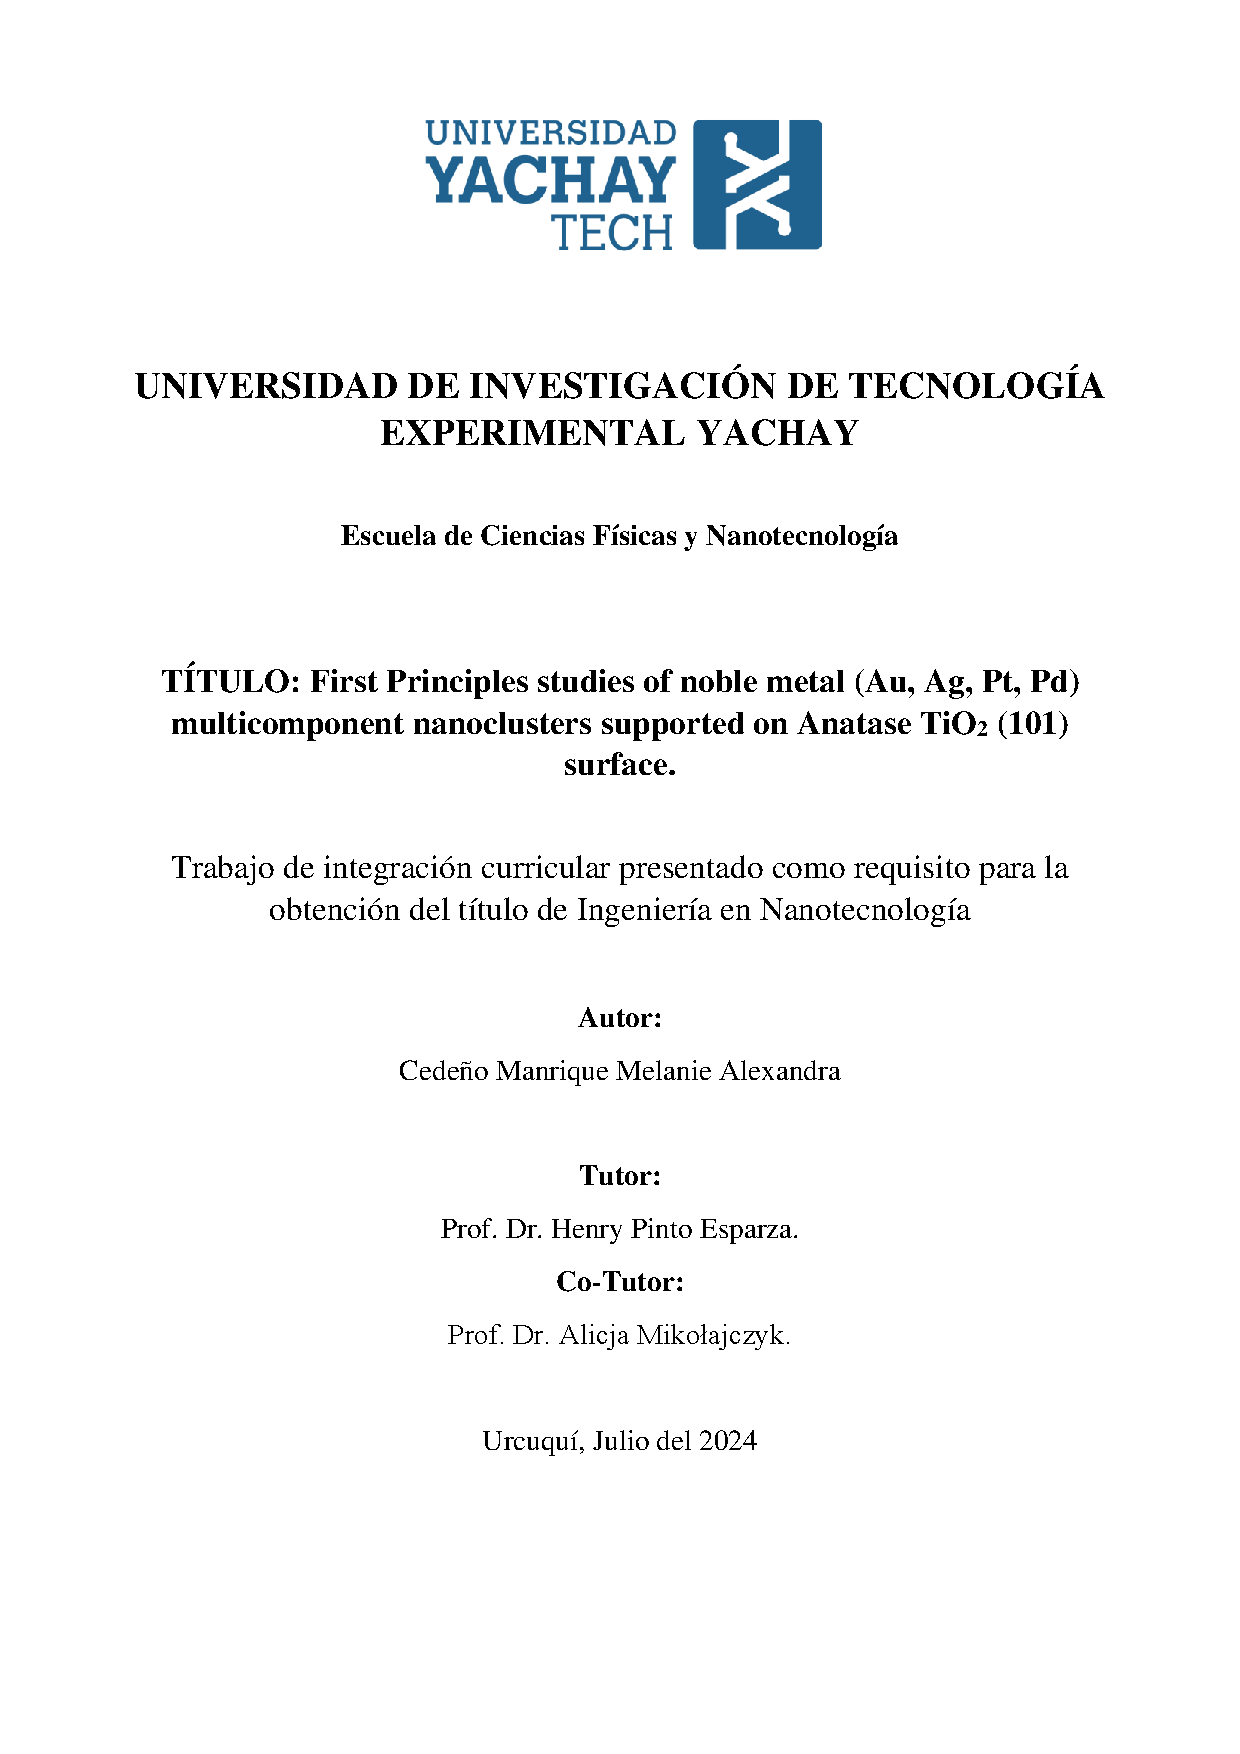
\includepdf[pages=-]{Caratula.pdf}
%\edeclarationpage

\let\cleardoublepage\clearpage
%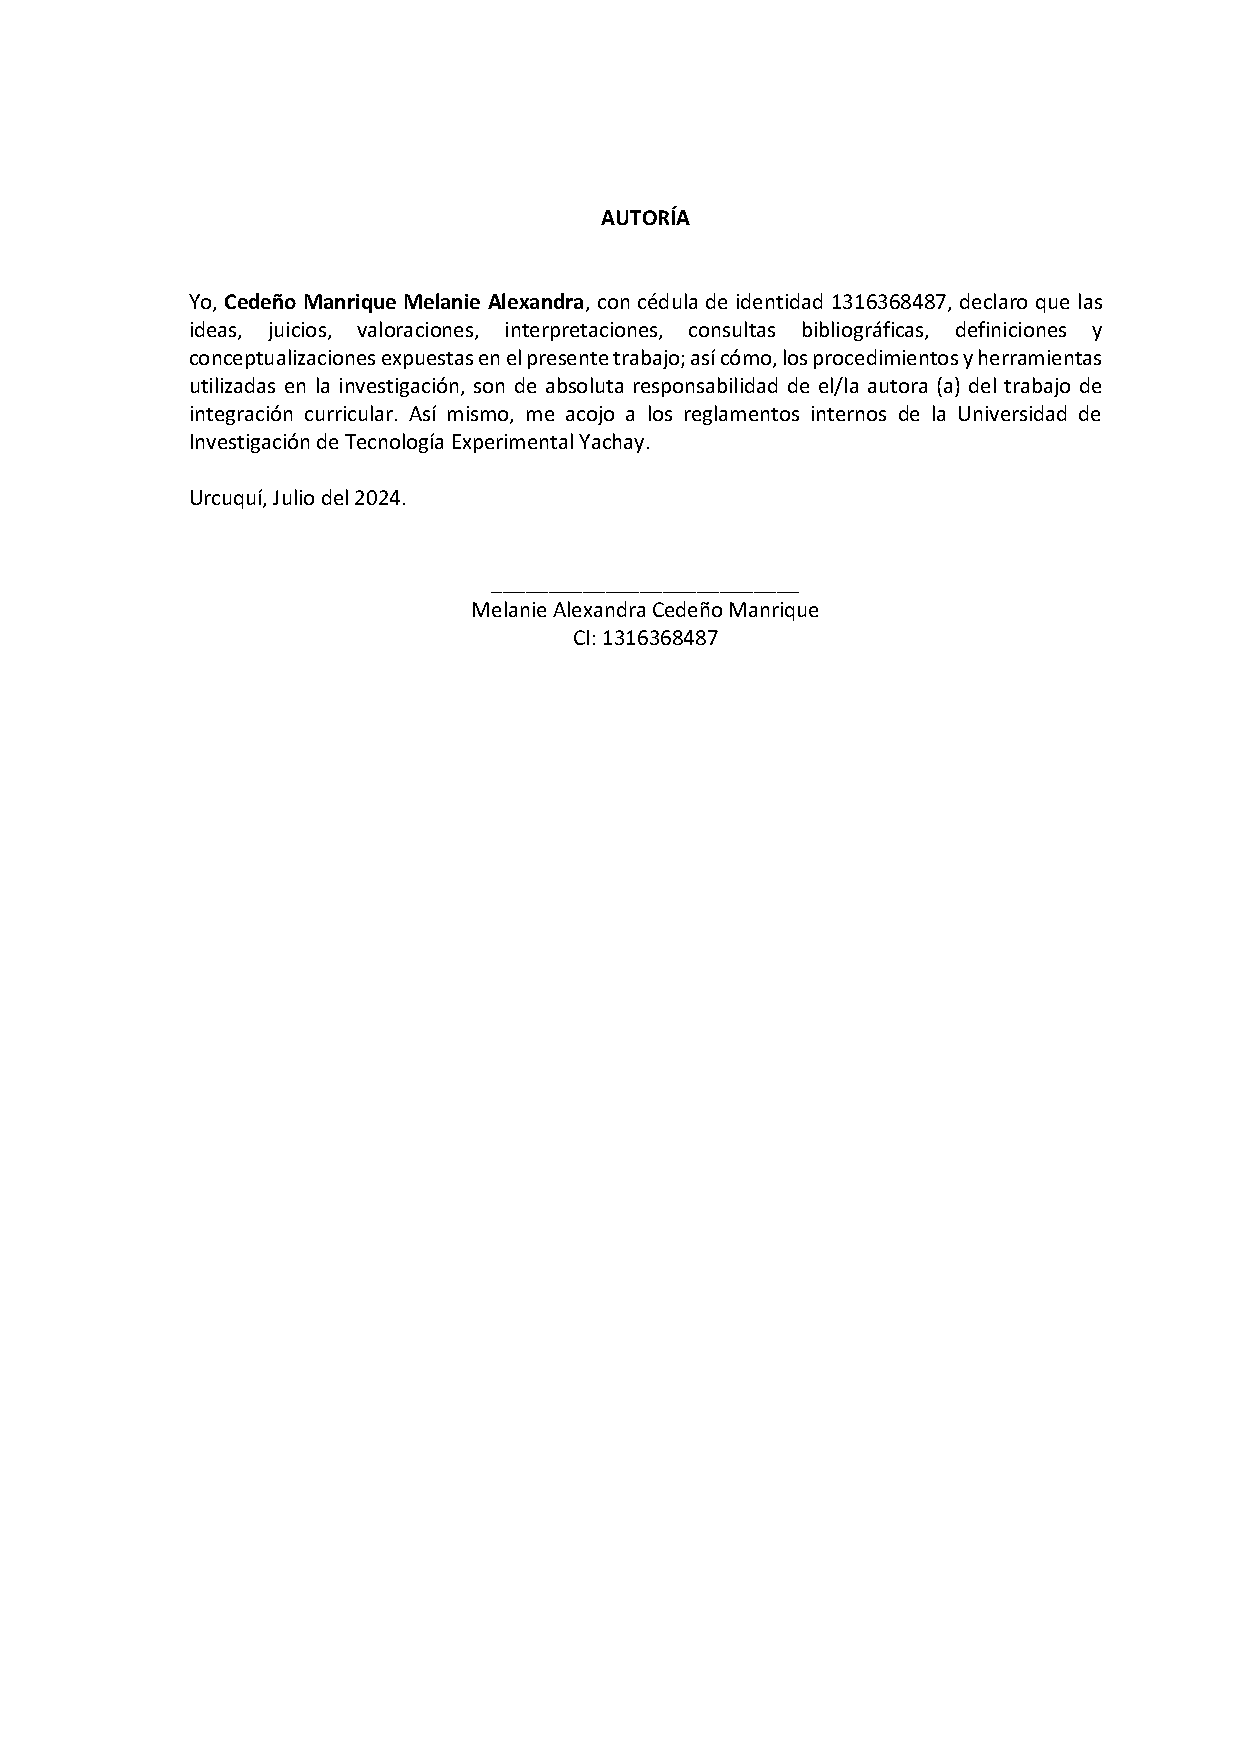
\includepdf[pages=-]{AUTORÍA-signed.pdf}
%
\includepdf[pages=1]{AUTORIZACIÓN DE PUBLICACIÓN-signed.pdf}

%############################# Dedication #################################
%\begin{dedication}
\chapter*{}
  \begin{center}
\fontsize{12}{15}\selectfont \textit{Insert here a dedication to someone or something.}
\vfill
  \end{center}


%############################# Acknowledgments #################################
\begin{acknowledgements}
Here you can write your acknowledgments 
\end{acknowledgements}

%############################# Abstract #################################
\begin{Resumen}
El concreto es la segunda sustancia más utilizada en el mundo después del agua, con más de 35 mil millones de toneladas producidas cada año. Sin embargo, comprender las propiedades atómicas y mecánicas del principal componente del concreto, los hidratos de cemento de silicato de calcio (C-S-H), la fase aglutinante compleja del concreto, sigue siendo un desafío.

En este proyecto, nuestro objetivo es investigar las propiedades atómicas y mecánicas de los hidratos de cemento utilizando teoría de funcionales de densidad (DFT) y herramientas de aprendizaje automático (ML). Comenzaremos utilizando DFT para estudiar la estructura electrónica, los enlaces y las respuestas mecánicas de C-S-H a nivel atómico. Posteriormente, utilizaremos dinámica molecular \emph{ab initio} (AIMD) junto con ML para crear un campo de fuerza en tiempo real de C-S-H, lo que nos permitirá simular con precisión y capturar las complejas interacciones atómicas de los hidratos de cemento, reduciendo al mismo tiempo el tiempo de cálculo. Al integrar DFT, AIMD y ML, buscamos proporcionar una comprensión más profunda de las propiedades fundamentales de C-S-H y desarrollar un modelo predictivo que pueda orientar el diseño de materiales de concreto más sostenibles y duraderos. 
 \\
 \\
 \emph{\textbf{Palabras clave:}}
\end{Resumen}

\begin{abstract} 
Concrete is the second-most-used substance in the world after water, with more than 35 billion tons produced, every year. Yet, understanding the atomic and mechanical properties of the main component of concrete, calcium-silicate-hydrate (C-S-H) cement hydrates--the complex binder phase of concrete---still poses a challenge.
  
In this project, we aim to investigate the atomic and mechanical properties of cement hydrates leveraging density-functional theory (DFT) and machine learning (ML) tools. We will first start by using DFT to study the electronic structure, bonding, and mechanical responses of C-S-H  at the atomic level. Afterwards, we will use \emph{ab initio} molecular dynamics (AIMD) with ML to create a force field on the fly of C-S-H, which will allow us to accurately simulate and capture the complex atomic interactions of cement hydrates while reducing the computation time. By integrating both DFT, AIMD and ML, we seek to provide deeper insights into the fundamental properties of C-S-H and to develop a predictive model that could inform the design of more sustainable and durable concrete materials.
 \\
  \\
 \emph{\textbf{Keywords:}}
\end{abstract}

\tableofcontents
\addcontentsline{toc}{chapter}{List of Figures}
\listoffigures
\addcontentsline{toc}{chapter}{List of Tables}
\listoftables
\addcontentsline{toc}{chapter}{List of Papers}


\mainbody
%############################# Introduction #################################
\chapter{Introduction}\label{Introduction}\glsresetall 

  \section{Background}\label{Background} 
  Concrete is the synthetic material currently produced in volumes larger than any other material on Earth. With an annual consumption of approximately 35 billion tonnes, it is only second to water in terms of global usage\cite{Monteiro2017, VanDamme2018}. As the backbone of modern infrastructure, it provides the foundations for buildings, bridges, roads, dams, and other structures essential for societal development. Its widespread adoption arises from a unique combination of strength, versatility, and cost-effectiveness\cite{Mehta2014}, rendering it indispensable to the construction industry.


  Nevertheless, despite the ubiquity of concrete, the properties of its key constituent, cement, remain incompletely understood. Cement is a chemically complex material, composed of a heterogeneous mixture of minerals that undergo a series of hydration reactions upon contact with water. The principal product of cement hydration---and the primary binding phase of concrete--- calcium silicate hydrate (C-S-H) is the responsible for the mechanical strength, chemical and transport properties and durability of hardened cement paste and, consequently, of concrete itself\cite{Papatzani2015, Qomi2020, Bahraq2022}. Therefore, understanding the atomic and mechanical properties of C-S-H is of the uttermost importance for the development of featured cementitious materials with enhanced performance and durability. 



%insert a figure 
  \begin{figure}[H]
    \centering
    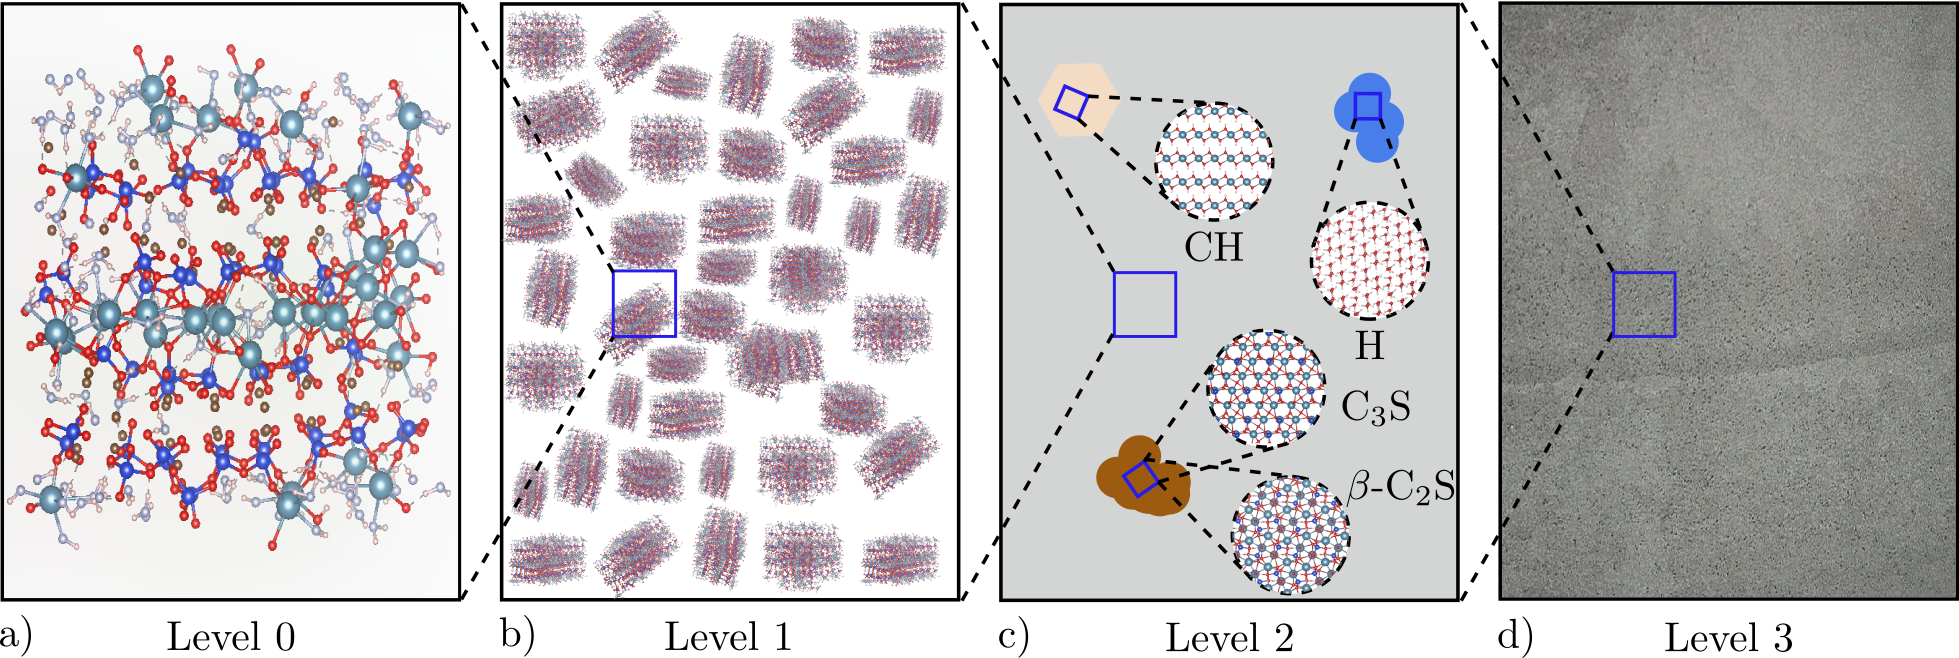
\includegraphics[width=1\textwidth]{levels.png}
    \caption{Caption}
    \label{fig:C-S-H}
  \end{figure}


  \section{Problem Statement}\label{Problem Statement}


  \section{Objectives}\label{Objectives}
  
  \subsection{General Objective}\label{General Objective}

  \subsection{Specific Objectives}\label{Specific Objectives}



\chapter{Theoretical Background}\label{Theoretical Background}

\section{Many-Body Schrödinger Equation}\label{Many Body Schrödinger Equation}

\section{The Born-Oppenheimer Approximation}\label{The Born-Oppenheimer Approximation}

\section{Density Functional Theory}\label{Density Functional Theory}









\bibliography{./thesis_project}
\bibliographystyle{thesis}
\printglossary[type=\acronymtype, title={Abbreviations}]

\end{document}
